\documentclass[12pt]{ctexart}
\usepackage{graphicx}
\usepackage{float} 
\usepackage{subfigure}
\usepackage[]{caption2}
\renewcommand{\figurename}{\textbf{Fig.}} %重定义编号前缀词
\renewcommand{\captionlabeldelim}{.~} %重定义分隔符,将默认的分隔符(通常是冒号 : 或其他字符)更改为一个点 . 后跟一个小空格 ~(在 LaTeX 中 ~ 代表一个不断行的空格)。
%\roman是罗马数字编号,\alph是默认的字母编号,\arabic是阿拉伯数字编号,可按需替换下一行的相应位置
\renewcommand{\thesubfigure}{(\roman{subfigure})} % 这行代码将子图编号设置为罗马数字,并且在编号外加括号。
\makeatletter \renewcommand{\@thesubfigure}{\thesubfigure \space} % 子图编号与名称的间隔设置。这里是加了一个空格:\space
\renewcommand{\p@subfigure}{} \makeatother % 重定义子图的引用格式,此处是清除了前缀,因此在引用时只显示子图编号,不显示主图编号。

\begin{document}
Figure \ref{Fig.main} 
has two sub figures, 
fig. \ref{Fig.sub.1} is the travel demand of driving auto,
and fig. \ref{Fig.sub.2} is the travel demand of park-and-ride.

\begin{figure}[htbp]
    \centering  %图片全局居中
    \subfigure[子图1标题]{
        \label{Fig.sub.1}%子图1索引
        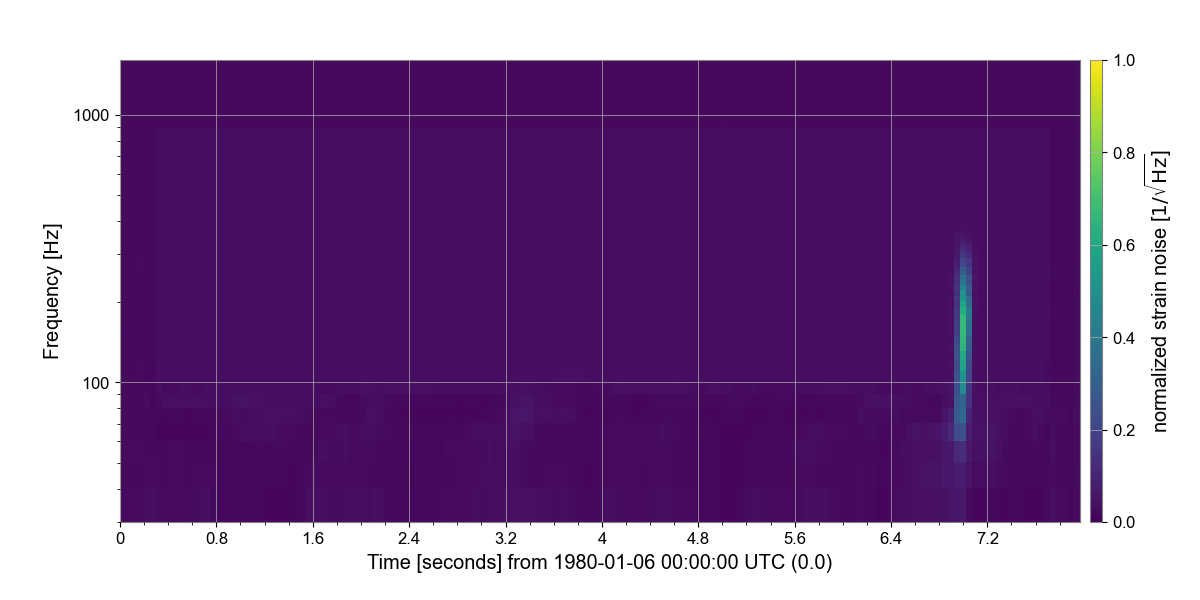
\includegraphics[width=0.45\textwidth]{image_p1.png}}%子图1文件名
    \subfigure[子图2标题]{%如果把\subfigure[子图2标题]{变为\subfigure{},就可以不显示子图的标题和编号.
        \label{Fig.sub.2}
        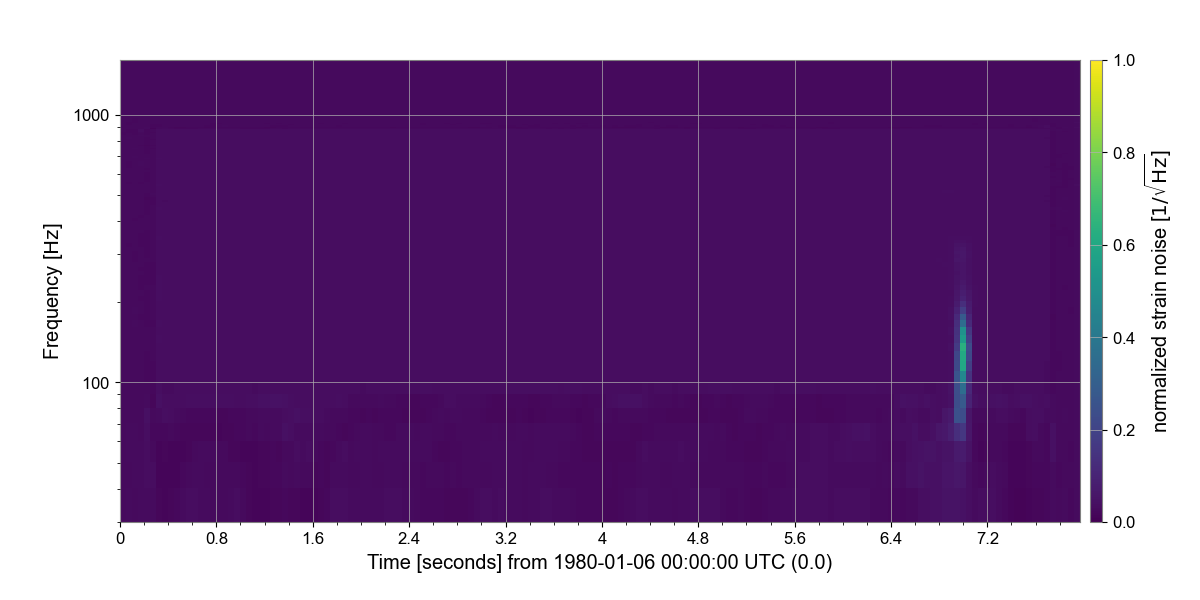
\includegraphics[width=0.45\textwidth]{image_p2.png}}%子图1文件名
    \caption{主图标题}
    \label{Fig.main}%主图索引
\end{figure}
\end{document}
